\chapter{Analiza și proiectarea sistemului}

\section{Arhitectura de ansamblu}

Pentru a asigura modularitatea, mentenanța facilă și securitatea resurselor, platforma a fost proiectată pe baza unei arhitecturi client-server decuplate. Server-ul din backend preia rolul de orchestrator central, gestionând regulile de business și coordonând serviciile specializate de execuție de cod și inteligență artificială. 

Sistemul este divizat în patru straturi distincte, interconectate prin protocoale standard de rețea:

\begin{enumerate}
    \item Nivelul de prezentare (Frontend): Implementat în React și TypeScript, responsabil de interacțiunea directă cu utilizatorul, afișarea enunțurilor în Markdown și capturarea soluțiilor la problemele algoritmice.
    \item Nivelul de orchestrare și logică (Backend): Dezvoltat în Spring Boot, centralizează logica aplicației, autentificarea securizată, gestiunea economiei virtuale (experiență, monede), resetarea provocărilor zilnice și a clasamentului lunar și autorizarea pe bază de roluri (utilizator, creator, moderator și administrator).
    \item Nivelul de persistență (Baza de date): Realizat în PostgreSQL pentru stocarea stării globale a sistemului: utilizatori, probleme de algoritmică, chestionare, submisii, relații de prietenie, mesaje, notificări. 
    \item Nivelul serviciilor specializate (Sandbox și LLM): Compus din motorul local Judge0 pentru compilarea și executarea izolată a codului și mediul Ollama (Qwen2.5-coder) pentru generarea chestionarelor și a răspunsurilor greșite.
\end{enumerate}

O ilustrare grafică a acestor componente se regăsește în Figura 3.1.

\begin{figure}[ht]
    \centering
    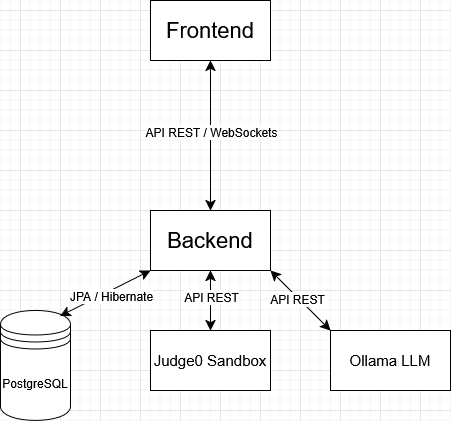
\includegraphics[width=0.8\textwidth]{diagrama arhitectura.png}
    \caption{Arhitectura de ansamblu a platformei}
    \label{fig:architecture}
\end{figure}

\section{Modelul conceptual al datelor}

Persistența datelor este structurată relațional în PostgreSQL, fiind optimizată pentru a suporta interogări frecvente și relații complexe între modulele sociale și cele algoritmice. Structura bazei de date este reprezentată de următoarele entități nucleu:

\begin{itemize}
    \item Account: stochează credențialele, hash-ul parolei, rolul de acces (utilizator, creator, moderator, administrator), nivelul de experiență, balanța de monede și detaliile de profil. 
    \item Problem și Submission: modelează ierarhia problemelor algoritmice (incluzând metadate precum dificultatea și vizibilitatea) și stochează istoricul încercărilor de rezolvare trimise de utilizatori către motorul de evaluare.
    \item Quiz: păstrează structura chestionarelor generate automat, incluzând secvența de cod, limbajul (C++ sau Python), răspunsul corect și variantele de răspuns plauzibile. 
    \item Friendship, Message și Post: gestionează rețeaua socială a platformei, de la stabilirea conexiunilor între conturi, până la schimbul de mesaje directe și publicarea de conținut. 
    \item Streak: monitorizează activitatea utilizatorului, contorizând atât seriile zilnice individuale (prin rezolvarea problemei zilei), cât și pe cele colaborative dintre prieteni (prin rezolvarea chestionarului zilnic) 
\end{itemize}

Pentru a menține performanța bazei de date și a evita timpii mari de răspuns, fișierele masive (scripturile de validare și fișierele cu seturile de date de intrare și ieșire) nu sunt stocate intern ca obiecte binare de mari dimensiuni (BLOB – Binary Large Object). Persistența lor se realizează în sistemul de fișiere al serverului, în timp ce tabelele stochează căile către aceste locații pe disc.

Ilustrarea grafică a acestor entități se află în Figura 3.2.

\begin{figure}[ht]
    \centering
    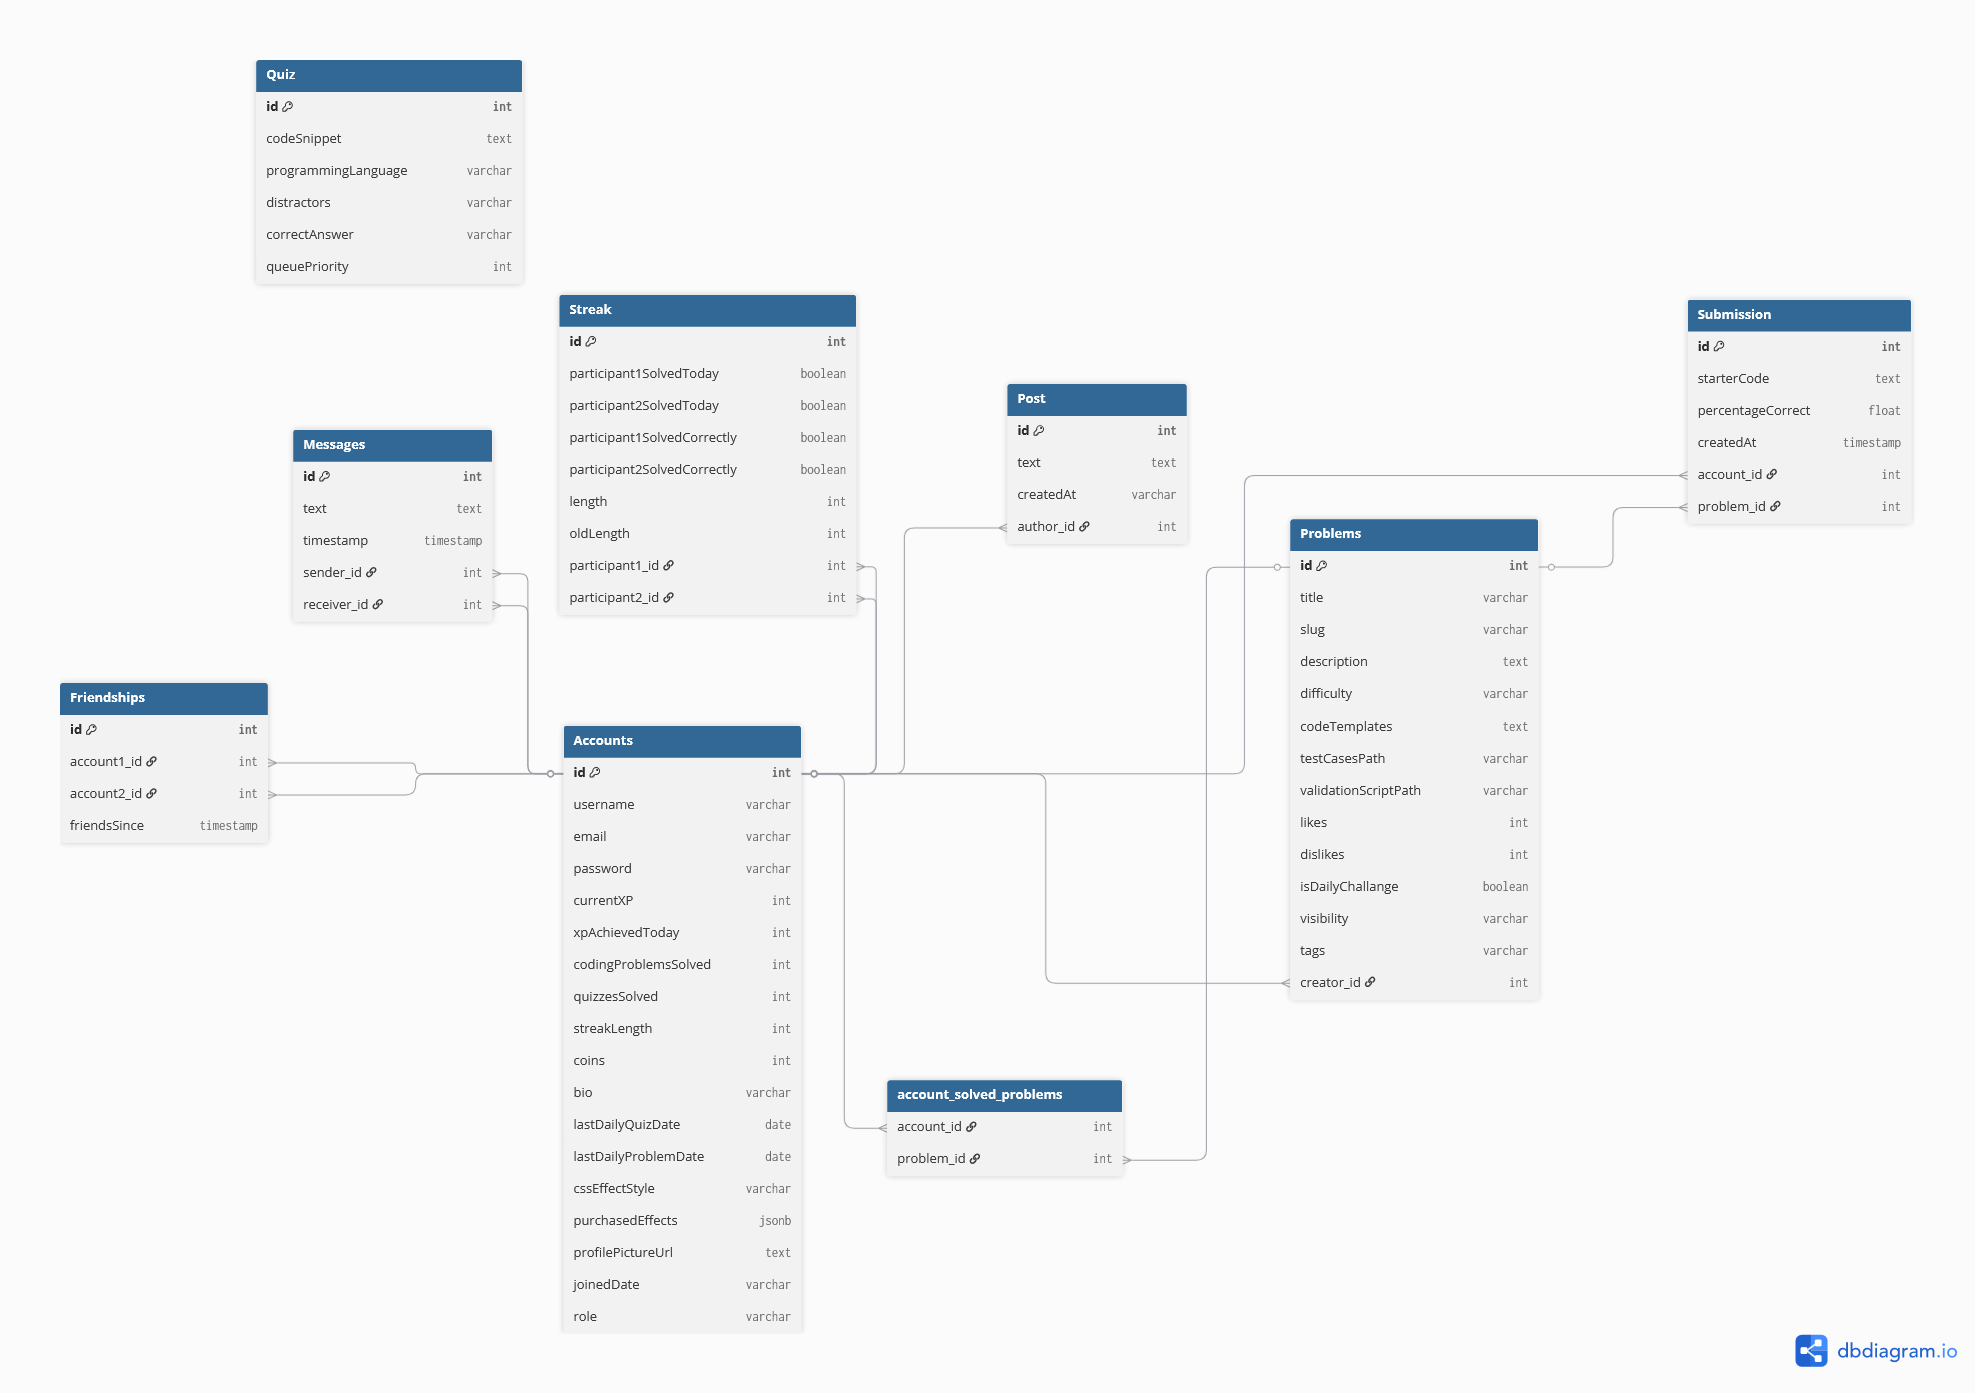
\includegraphics[width=1\textwidth]{erd.png}
    \caption{Arhitectura de ansamblu a platformei}
    \label{fig:erd}
\end{figure}